
\section{Access Security.
Authentication}
\label{sec:sec:auth}

For a user to be able to create processes for using a computer system, they must authenticate, that is, certify an \textbf{identity} that can access the system.
In the absence of authentication, a user cannot use a computer system.
This prevents unauthorized users from accessing the system.

Authentication involves transmitting authentication information usually composed of a username (\textit{username}) and an authentication element (\textit{authentication token}), often a password.
This is the form described in \labelindexref{Section}{sec:user:auth}.
Besides passwords, a user can use biometric data (such as fingerprint, common on laptops or mobile phones, facial recognition, such as that used by iPhoneX or retina recognition), can use public key authentication or digital certificates, or can use a hardware device (such as tokens used for authentication in online bank accounts).
Hardware devices (\textit{hardware tokens}) or applications on mobile devices use one-time passwords (\textit{one-time passwords}).
These are passwords that expire in a short time, after the expiration of one password, a new one is generated.
In this way, an attacker's retention of a password is prevented.

As specified in \labelindexref{Figure}{fig:sec:password-auth-hashing}, within the authentication process, a user transmits a username and an authentication element.
The system has an \textbf{authentication database} (\textit{authentication database}) which it consults and sees if there is an entry for the provided username with the corresponding authentication element.
Access is permitted if both are found in the authentication database.
Otherwise, access is blocked.

For the case where we have multiple services (which can be located on multiple systems) that use the same username and authentication element, we can use centralized authentication, as we presented in \labelindexref{Section}{sec:user:centralized-auth}.
In this situation, the authentication database is managed by a dedicated service that is contacted when we want authentication for another service.

For increasing the security level in case of authentication, we can use \textbf{multi-factor authentication} (\textit{multi-factor authentication}).
The usual form is \textbf{two-factor authentication} (2FA).
In this case, multiple authentication methods are used: a password and a one-time password or a password and a biometric identifier.
We recommend that, for sensitive services (such as email, social networks, data storage services), you use multi-factor authentication.

\subsection{Password Management}
\label{sec:sec:auth:password}

The most common authentication element is represented by passwords.
Passwords are character strings provided to the authentication system to certify the user's identity.
Passwords must be kept private, otherwise an attacker will impersonate a user and authenticate into the system claiming to be them.
That is why passwords must be managed carefully.

Passwords must be stored in the authentication database described in \labelindexref{Section}{sec:user:password-db}.
It is problematic for passwords to be stored in readable format (\textit{plaintext}).
If the database is compromised, an attacker will have access to all users' passwords.
That is why, in general, passwords are not stored in plaintext format in the database, but a summary of them is stored, obtained with the help of a hashing algorithm as we described in \labelindexref{Section}{sec:sec:data:integrity}.
Hashing algorithms are called one-way algorithms because we can quickly obtain the summary of a message (in this case a password), but the function is not reversible.
Thus, for authentication in a system, the steps below are followed, also described in \labelindexref{Figure}{fig:sec:password-auth-hashing}.

\begin{enumerate}
  \item The user who wants authentication provides a username and password.
  \item The hashing algorithm is applied to the password and the summary is obtained.
  \item The database is searched for the entry composed of the username and the message summary.
    If such an entry is found, the user is permitted access to the system.
\end{enumerate}

\begin{figure}[htbp]
  \centering
  \def\svgwidth{\columnwidth}
  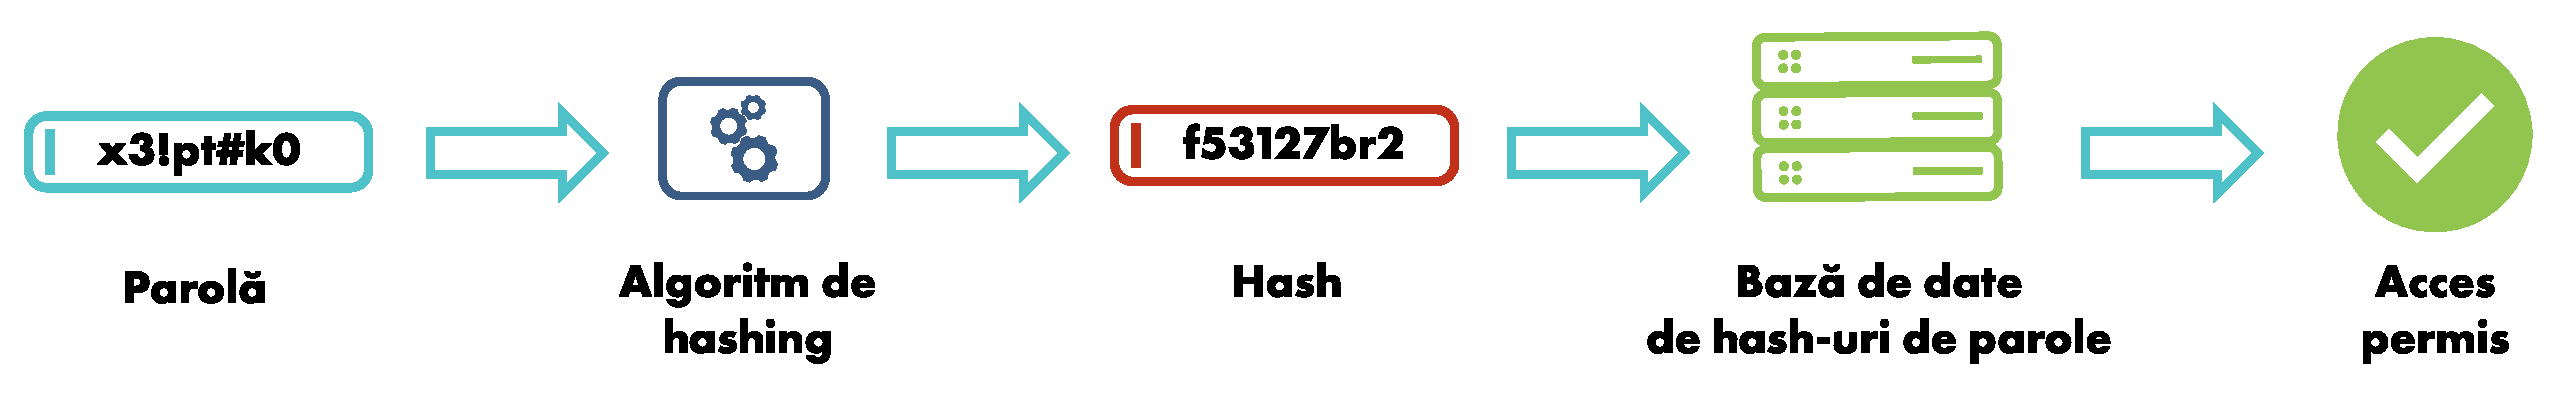
\includegraphics{chapters/12-auth/img/password-auth-hashing.svg.pdf}
  \caption{Password Authentication}
  \label{fig:sec:password-auth-hashing}
\end{figure}

Even if the password is not stored in plaintext format in the database, but as a summary, access to the database must be restricted.
This is a form of the defense in depth principle.
In Linux, as we presented in \labelindexref{Section}{sec:user:password-db}, user information is stored in the file \file{/etc/passwd} which is readable by all users.
However, password information is stored in the file \file{/etc/shadow} which is readable only by privileged processes.
In addition, in the file \file{/etc/shadow} passwords are stored as summaries, not in plaintext format.

Obtaining a password is, for an attacker, the way to gain access to the system.
They can obtain the password either from the user or their actions (social engineering, message capture, finding the password written on a paper or in an accessible file, blackmail, threat) or can try guessing or finding the password directly from the authentication system.
We call the last approach \textbf{password/account cracking} (\textit{password cracking}).
Password cracking has two forms:

\begin{enumerate}
  \item \textit{Online password cracking}: the attacker tries passwords one by one and asks the authentication system to validate if the password is correct.
  \item \textit{Offline password cracking}: the attacker gains access to the password database (stored in summary format) and calculates password summaries to compare them with those in the database.
\end{enumerate}

There are dedicated utilities to assist in password cracking.
Utilities such as THC-Hydra\footnote{\url{https://github.com/vanhauser-thc/thc-hydra}} or Burp Suite\footnote{\url{https://portswigger.net/burp}} are used for online password cracking, while utilities such as John the Ripper\footnote{\url{https://www.openwall.com/john/}} are used for offline password cracking.
The Crackstation website\footnote{\url{https://crackstation.net/}} offers the offline password cracking service, with the user having to provide password summaries so that it can report if it has the initial password.
The advantage of online password cracking is that it does not require access to the password database (i.e., there must be a \textit{password leak} type attack beforehand).
But not many passwords can be tested per second, as in the case of offline password cracking;
in addition, a system will report the situation or will deactivate in case of a large number of failed attempts per second.

Passwords remain the main form of authentication for many services on the Internet.
In such an interconnected world, the risks of an attacker discovering the password in the ways described above are high.
That is why there are recommendations for generating, using, and managing passwords such as those described below.
Many organizations establish and apply password usage policies to minimize the risk of their discovery and to prevent attackers from accessing the organization's resources:

\begin{itemize}
  \item Passwords should contain as wide a set of characters as possible, not just lowercase letters.
    They can contain uppercase letters, digits, punctuation marks.
  \item Passwords must have a length of over 10-12 characters.
    Passwords with smaller size can be guessed or cracked.
    The use of passphrases is ideal, that is, passwords composed of words, ideally unrelated to each other, harder to guess and easier to remember.
    As described in a famous xkcd illustration\footnote{\url{https://xkcd.com/936/}}, a password like \texttt{Tr0oub4dor\&3} is harder to remember and easier to crack than the passphrase \texttt{correct horse battery staple}.
  \item The use of multi-factor authentication is recommended.
    Generally, the mobile phone is used (SMS sending or applications like Google Authenticator) as an additional form of authentication, not just passwords.
    In this way, if someone obtains the password, they will not be able to access the service without access to the user's mobile phone.
    In addition, the user will be notified of the authentication attempt.
  \item Passwords should be changed periodically.
    It is ideal for a password to be changed once every 6-12 months.
    If it has been cracked/guessed, the password will become useless once it has been changed.
\end{itemize}

Nowadays, we have many services that we access based on passwords: desktop system, email, online shopping, online media, social networks, storage services, financial services.
There is a risk that we end up using a password two or more times on the same site/service.
It is important to use different passwords for different services.
If a password is guessed, access to a single service is compromised.

Given the large number of passwords used, different and hard-to-guess passwords or passphrases must be generated.
For this, it is useful to turn to \textbf{password generators}.
Modern web browsers have integrated password generators that will automatically fill in the fields in web forms for creating accounts and passwords.
Besides these, we can use Linux utilities for password generation, such as \cmd{pwgen}, \cmd{apg}, or \cmd{xkcdpass}, or we can use a password manager.

For managing and storing passwords, the use of a \cmd{password manager} (\textit{password manager}) is recommended.
A password manager stores information about the service/site used and the corresponding password and encrypts this information.
A master password (\textit{master password}) is needed to access them.
Password managers can be applications that work only locally (such as UPM, KeePass, or PasswordGorrila) or others that store information in the cloud, allowing their sharing between different devices (such as LastPass, Dashlane, or Keeper).
Besides secure password storage, password managers offer functionalities such as password generation, automatic form filling, password sharing between multiple accounts.

Passwords are a critical component in users' access to devices and services on the Internet.
That is why they must be protected by those who design and administer systems and must be managed carefully by every user.
The large number of sites and services that we use with the help of passwords increases the risk of losing them, and recommendations such as those above must be followed for their management.
